% Options for packages loaded elsewhere
\PassOptionsToPackage{unicode}{hyperref}
\PassOptionsToPackage{hyphens}{url}
\PassOptionsToPackage{dvipsnames,svgnames,x11names}{xcolor}
%
\documentclass[
  letterpaper,
  DIV=11,
  numbers=noendperiod]{scrartcl}

\usepackage{amsmath,amssymb}
\usepackage{iftex}
\ifPDFTeX
  \usepackage[T1]{fontenc}
  \usepackage[utf8]{inputenc}
  \usepackage{textcomp} % provide euro and other symbols
\else % if luatex or xetex
  \usepackage{unicode-math}
  \defaultfontfeatures{Scale=MatchLowercase}
  \defaultfontfeatures[\rmfamily]{Ligatures=TeX,Scale=1}
\fi
\usepackage{lmodern}
\ifPDFTeX\else  
    % xetex/luatex font selection
\fi
% Use upquote if available, for straight quotes in verbatim environments
\IfFileExists{upquote.sty}{\usepackage{upquote}}{}
\IfFileExists{microtype.sty}{% use microtype if available
  \usepackage[]{microtype}
  \UseMicrotypeSet[protrusion]{basicmath} % disable protrusion for tt fonts
}{}
\makeatletter
\@ifundefined{KOMAClassName}{% if non-KOMA class
  \IfFileExists{parskip.sty}{%
    \usepackage{parskip}
  }{% else
    \setlength{\parindent}{0pt}
    \setlength{\parskip}{6pt plus 2pt minus 1pt}}
}{% if KOMA class
  \KOMAoptions{parskip=half}}
\makeatother
\usepackage{xcolor}
\setlength{\emergencystretch}{3em} % prevent overfull lines
\setcounter{secnumdepth}{-\maxdimen} % remove section numbering
% Make \paragraph and \subparagraph free-standing
\ifx\paragraph\undefined\else
  \let\oldparagraph\paragraph
  \renewcommand{\paragraph}[1]{\oldparagraph{#1}\mbox{}}
\fi
\ifx\subparagraph\undefined\else
  \let\oldsubparagraph\subparagraph
  \renewcommand{\subparagraph}[1]{\oldsubparagraph{#1}\mbox{}}
\fi

\usepackage{color}
\usepackage{fancyvrb}
\newcommand{\VerbBar}{|}
\newcommand{\VERB}{\Verb[commandchars=\\\{\}]}
\DefineVerbatimEnvironment{Highlighting}{Verbatim}{commandchars=\\\{\}}
% Add ',fontsize=\small' for more characters per line
\usepackage{framed}
\definecolor{shadecolor}{RGB}{241,243,245}
\newenvironment{Shaded}{\begin{snugshade}}{\end{snugshade}}
\newcommand{\AlertTok}[1]{\textcolor[rgb]{0.68,0.00,0.00}{#1}}
\newcommand{\AnnotationTok}[1]{\textcolor[rgb]{0.37,0.37,0.37}{#1}}
\newcommand{\AttributeTok}[1]{\textcolor[rgb]{0.40,0.45,0.13}{#1}}
\newcommand{\BaseNTok}[1]{\textcolor[rgb]{0.68,0.00,0.00}{#1}}
\newcommand{\BuiltInTok}[1]{\textcolor[rgb]{0.00,0.23,0.31}{#1}}
\newcommand{\CharTok}[1]{\textcolor[rgb]{0.13,0.47,0.30}{#1}}
\newcommand{\CommentTok}[1]{\textcolor[rgb]{0.37,0.37,0.37}{#1}}
\newcommand{\CommentVarTok}[1]{\textcolor[rgb]{0.37,0.37,0.37}{\textit{#1}}}
\newcommand{\ConstantTok}[1]{\textcolor[rgb]{0.56,0.35,0.01}{#1}}
\newcommand{\ControlFlowTok}[1]{\textcolor[rgb]{0.00,0.23,0.31}{#1}}
\newcommand{\DataTypeTok}[1]{\textcolor[rgb]{0.68,0.00,0.00}{#1}}
\newcommand{\DecValTok}[1]{\textcolor[rgb]{0.68,0.00,0.00}{#1}}
\newcommand{\DocumentationTok}[1]{\textcolor[rgb]{0.37,0.37,0.37}{\textit{#1}}}
\newcommand{\ErrorTok}[1]{\textcolor[rgb]{0.68,0.00,0.00}{#1}}
\newcommand{\ExtensionTok}[1]{\textcolor[rgb]{0.00,0.23,0.31}{#1}}
\newcommand{\FloatTok}[1]{\textcolor[rgb]{0.68,0.00,0.00}{#1}}
\newcommand{\FunctionTok}[1]{\textcolor[rgb]{0.28,0.35,0.67}{#1}}
\newcommand{\ImportTok}[1]{\textcolor[rgb]{0.00,0.46,0.62}{#1}}
\newcommand{\InformationTok}[1]{\textcolor[rgb]{0.37,0.37,0.37}{#1}}
\newcommand{\KeywordTok}[1]{\textcolor[rgb]{0.00,0.23,0.31}{#1}}
\newcommand{\NormalTok}[1]{\textcolor[rgb]{0.00,0.23,0.31}{#1}}
\newcommand{\OperatorTok}[1]{\textcolor[rgb]{0.37,0.37,0.37}{#1}}
\newcommand{\OtherTok}[1]{\textcolor[rgb]{0.00,0.23,0.31}{#1}}
\newcommand{\PreprocessorTok}[1]{\textcolor[rgb]{0.68,0.00,0.00}{#1}}
\newcommand{\RegionMarkerTok}[1]{\textcolor[rgb]{0.00,0.23,0.31}{#1}}
\newcommand{\SpecialCharTok}[1]{\textcolor[rgb]{0.37,0.37,0.37}{#1}}
\newcommand{\SpecialStringTok}[1]{\textcolor[rgb]{0.13,0.47,0.30}{#1}}
\newcommand{\StringTok}[1]{\textcolor[rgb]{0.13,0.47,0.30}{#1}}
\newcommand{\VariableTok}[1]{\textcolor[rgb]{0.07,0.07,0.07}{#1}}
\newcommand{\VerbatimStringTok}[1]{\textcolor[rgb]{0.13,0.47,0.30}{#1}}
\newcommand{\WarningTok}[1]{\textcolor[rgb]{0.37,0.37,0.37}{\textit{#1}}}

\providecommand{\tightlist}{%
  \setlength{\itemsep}{0pt}\setlength{\parskip}{0pt}}\usepackage{longtable,booktabs,array}
\usepackage{calc} % for calculating minipage widths
% Correct order of tables after \paragraph or \subparagraph
\usepackage{etoolbox}
\makeatletter
\patchcmd\longtable{\par}{\if@noskipsec\mbox{}\fi\par}{}{}
\makeatother
% Allow footnotes in longtable head/foot
\IfFileExists{footnotehyper.sty}{\usepackage{footnotehyper}}{\usepackage{footnote}}
\makesavenoteenv{longtable}
\usepackage{graphicx}
\makeatletter
\def\maxwidth{\ifdim\Gin@nat@width>\linewidth\linewidth\else\Gin@nat@width\fi}
\def\maxheight{\ifdim\Gin@nat@height>\textheight\textheight\else\Gin@nat@height\fi}
\makeatother
% Scale images if necessary, so that they will not overflow the page
% margins by default, and it is still possible to overwrite the defaults
% using explicit options in \includegraphics[width, height, ...]{}
\setkeys{Gin}{width=\maxwidth,height=\maxheight,keepaspectratio}
% Set default figure placement to htbp
\makeatletter
\def\fps@figure{htbp}
\makeatother

\KOMAoption{captions}{tableheading}
\makeatletter
\makeatother
\makeatletter
\makeatother
\makeatletter
\@ifpackageloaded{caption}{}{\usepackage{caption}}
\AtBeginDocument{%
\ifdefined\contentsname
  \renewcommand*\contentsname{Table of contents}
\else
  \newcommand\contentsname{Table of contents}
\fi
\ifdefined\listfigurename
  \renewcommand*\listfigurename{List of Figures}
\else
  \newcommand\listfigurename{List of Figures}
\fi
\ifdefined\listtablename
  \renewcommand*\listtablename{List of Tables}
\else
  \newcommand\listtablename{List of Tables}
\fi
\ifdefined\figurename
  \renewcommand*\figurename{Figure}
\else
  \newcommand\figurename{Figure}
\fi
\ifdefined\tablename
  \renewcommand*\tablename{Table}
\else
  \newcommand\tablename{Table}
\fi
}
\@ifpackageloaded{float}{}{\usepackage{float}}
\floatstyle{ruled}
\@ifundefined{c@chapter}{\newfloat{codelisting}{h}{lop}}{\newfloat{codelisting}{h}{lop}[chapter]}
\floatname{codelisting}{Listing}
\newcommand*\listoflistings{\listof{codelisting}{List of Listings}}
\makeatother
\makeatletter
\@ifpackageloaded{caption}{}{\usepackage{caption}}
\@ifpackageloaded{subcaption}{}{\usepackage{subcaption}}
\makeatother
\makeatletter
\@ifpackageloaded{tcolorbox}{}{\usepackage[skins,breakable]{tcolorbox}}
\makeatother
\makeatletter
\@ifundefined{shadecolor}{\definecolor{shadecolor}{HTML}{FF0000}}
\makeatother
\makeatletter
\makeatother
\makeatletter
\makeatother
\ifLuaTeX
  \usepackage{selnolig}  % disable illegal ligatures
\fi
\IfFileExists{bookmark.sty}{\usepackage{bookmark}}{\usepackage{hyperref}}
\IfFileExists{xurl.sty}{\usepackage{xurl}}{} % add URL line breaks if available
\urlstyle{same} % disable monospaced font for URLs
\hypersetup{
  pdfauthor={Sebastián Egaña Santibáñez ; Nicolás Leiva Díaz },
  colorlinks=true,
  linkcolor={blue},
  filecolor={Maroon},
  citecolor={Blue},
  urlcolor={Blue},
  pdfcreator={LaTeX via pandoc}}

\title{Finanzas en R}
\usepackage{etoolbox}
\makeatletter
\providecommand{\subtitle}[1]{% add subtitle to \maketitle
  \apptocmd{\@title}{\par {\large #1 \par}}{}{}
}
\makeatother
\subtitle{Visualization}
\author{Sebastián Egaña Santibáñez
\href{mailto:segana@fen.uchile}{} \and Nicolás Leiva Díaz
\href{mailto:nleivad@fen.uchile.cl}{}}
\date{}

\begin{document}
\maketitle
\ifdefined\Shaded\renewenvironment{Shaded}{\begin{tcolorbox}[interior hidden, boxrule=0pt, enhanced, sharp corners, breakable, borderline west={3pt}{0pt}{shadecolor}, frame hidden]}{\end{tcolorbox}}\fi

-\/-\/-

\hypertarget{enlaces-del-profesor}{%
\section{Enlaces del profesor}\label{enlaces-del-profesor}}

\href{https://segana.netlify.app}{} https://segana.netlify.app

\href{https://github.com/sebaegana}{} https://github.com/sebaegana

\href{https://www.linkedin.com/in/sebastian-egana-santibanez/}{}
https://www.linkedin.com/in/sebastian-egana-santibanez/

\begin{center}\rule{0.5\linewidth}{0.5pt}\end{center}

\hypertarget{visualizaciuxf3n-en-r}{%
\section{Visualización en R}\label{visualizaciuxf3n-en-r}}

La principal librería para fines de visualización corresponde a GGPLOT2.
Crearemos un gráfico simple utilizando la librería ggplot2\footnote{Recordar
  instalar y cargar la librería}.

Revisemos el Cheatsheet asociado:

\href{https://github.com/rstudio/cheatsheets/blob/master/data-visualization-2.1.pdf}{Enlace acá}

La construcción de un gráfico utilizando GGPLOT2 se realiza a través de
los siguientes elementos:

\begin{enumerate}
\def\labelenumi{\arabic{enumi}.}
\tightlist
\item
  Un set de datos.
\item
  Un sistema de coordenadas.
\item
  Figuras geométricas (geoms) o representaciones visuales de los datos.
\end{enumerate}

Para cambiar la forma en que se muestran los datos se pueden editar las
figuras geométricas (geoms), cambiando color, tamaño y la ubicación de
los puntos en x y/o en y.

Inclusive se plantea una plantilla para esto:

\begin{verbatim}
ggplot (data = <DATA> ) +
 <GEOM_FUNCTION> (mapping = aes( <MAPPINGS> ),
 stat = <STAT> , position = <POSITION> ) +
 <COORDINATE_FUNCTION> +
 <FACET_FUNCTION> +
 <SCALE_FUNCTION> +
 <THEME_FUNCTION>
\end{verbatim}

En donde las dos primeras líneas son ogligatoias.

Apliquemos esto a los datos importados. Referencia relevante para esta
parte
\href{https://www.datanalytics.com/libro_r/elementos-de-un-grafico-en-ggplot2.html}{Enlace acá}

\begin{enumerate}
\def\labelenumi{\arabic{enumi}.}
\tightlist
\item
  Asignamos el set de datos:
\end{enumerate}

\begin{Shaded}
\begin{Highlighting}[]
\FunctionTok{library}\NormalTok{(tidyverse)}

\NormalTok{p }\OtherTok{\textless{}{-}} \FunctionTok{ggplot}\NormalTok{(data)}

\NormalTok{p}
\end{Highlighting}
\end{Shaded}

\begin{figure}[H]

{\centering 
\includegraphics{notebook_visualization_files/figure-pdf/unnamed-chunk-1-1.pdf}

}

\end{figure}

\begin{enumerate}
\def\labelenumi{\arabic{enumi}.}
\setcounter{enumi}{1}
\tightlist
\item
  Ahora declaramos el sistema de coordenadas:
\end{enumerate}

\begin{Shaded}
\begin{Highlighting}[]
\NormalTok{p }\OtherTok{\textless{}{-}} \FunctionTok{ggplot}\NormalTok{(data) }\SpecialCharTok{+} \FunctionTok{aes}\NormalTok{(}\AttributeTok{x =}\NormalTok{ sexo, }\AttributeTok{y =}\NormalTok{ fibe)}

\NormalTok{p}
\end{Highlighting}
\end{Shaded}

\begin{figure}[H]

{\centering 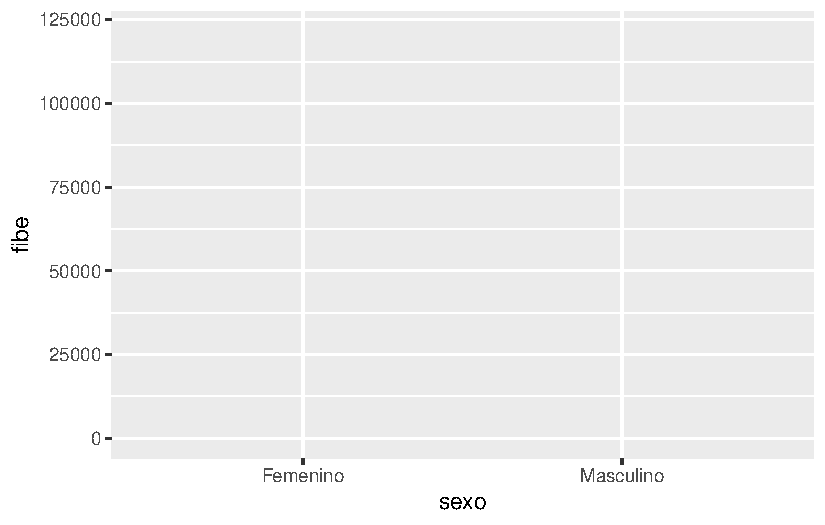
\includegraphics{notebook_visualization_files/figure-pdf/unnamed-chunk-2-1.pdf}

}

\end{figure}

\begin{itemize}
\tightlist
\item
  Cabe mencionar, que cada elemento que se agrega dentro de un gráfico
  en GGPLOT2, se realiza utilizando el signo ``+'' (cómo ir añadiendo
  capas).
\end{itemize}

\begin{enumerate}
\def\labelenumi{\arabic{enumi}.}
\setcounter{enumi}{2}
\tightlist
\item
  Declaremos ahora el tipo de figura, Por ejemplo, para un gráfico de
  barras el sistema de coordenadas solo debe contener el eje x (el eje y
  viene dado por el conteo de las ocurrencias):
\end{enumerate}

\begin{Shaded}
\begin{Highlighting}[]
\NormalTok{p }\OtherTok{\textless{}{-}} \FunctionTok{ggplot}\NormalTok{(data) }\SpecialCharTok{+} \FunctionTok{aes}\NormalTok{(}\AttributeTok{x =}\NormalTok{ sexo) }\SpecialCharTok{+} \FunctionTok{geom\_bar}\NormalTok{()}

\NormalTok{p}
\end{Highlighting}
\end{Shaded}

\begin{figure}[H]

{\centering 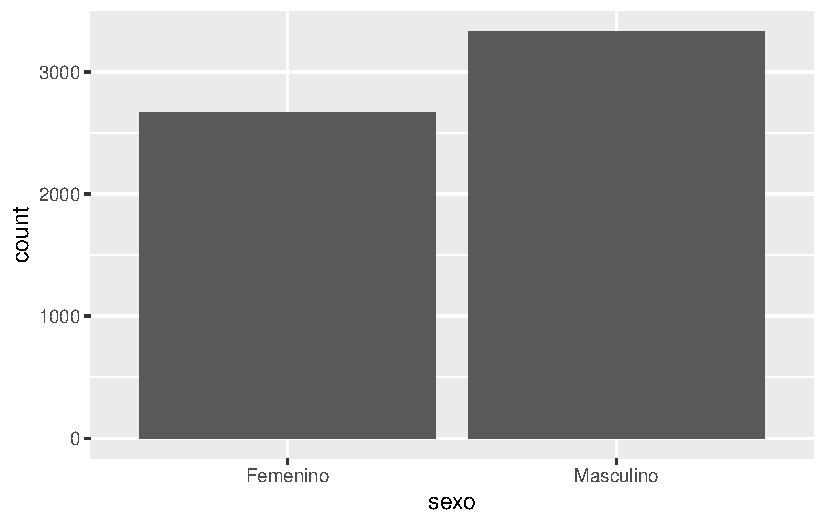
\includegraphics{notebook_visualization_files/figure-pdf/unnamed-chunk-3-1.pdf}

}

\end{figure}

Podemos voltear el gráfico, y agregar diferenciación en base a otra
variable:

\begin{Shaded}
\begin{Highlighting}[]
\NormalTok{p }\OtherTok{\textless{}{-}} \FunctionTok{ggplot}\NormalTok{(data) }\SpecialCharTok{+} \FunctionTok{aes}\NormalTok{(}\AttributeTok{y =}\NormalTok{ sexo) }\SpecialCharTok{+} \FunctionTok{geom\_bar}\NormalTok{(}\FunctionTok{aes}\NormalTok{(}\AttributeTok{fill =}\NormalTok{ afectacion))}

\NormalTok{p}
\end{Highlighting}
\end{Shaded}

\begin{figure}[H]

{\centering 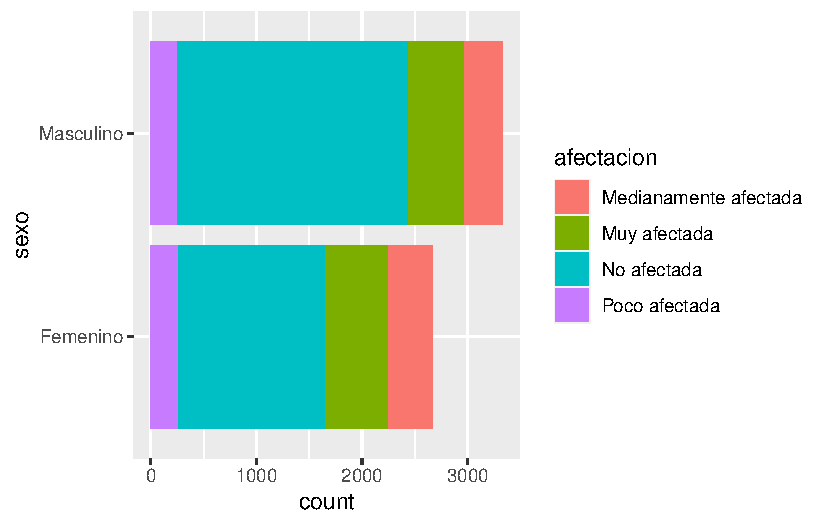
\includegraphics{notebook_visualization_files/figure-pdf/unnamed-chunk-4-1.pdf}

}

\end{figure}

Podríamos graficar de manera separada cada columna, en base a esta
página
\href{http://www.sthda.com/english/wiki/ggplot2-barplots-quick-start-guide-r-software-and-data-visualization}{Enlace acá}:

\begin{Shaded}
\begin{Highlighting}[]
\NormalTok{p }\OtherTok{\textless{}{-}} \FunctionTok{ggplot}\NormalTok{(data) }\SpecialCharTok{+} \FunctionTok{aes}\NormalTok{(}\AttributeTok{y =}\NormalTok{ sexo, }\AttributeTok{fill =}\NormalTok{ afectacion) }\SpecialCharTok{+} 
  \FunctionTok{geom\_bar}\NormalTok{(}\AttributeTok{position=}\FunctionTok{position\_dodge}\NormalTok{())}

\NormalTok{p}
\end{Highlighting}
\end{Shaded}

\begin{figure}[H]

{\centering 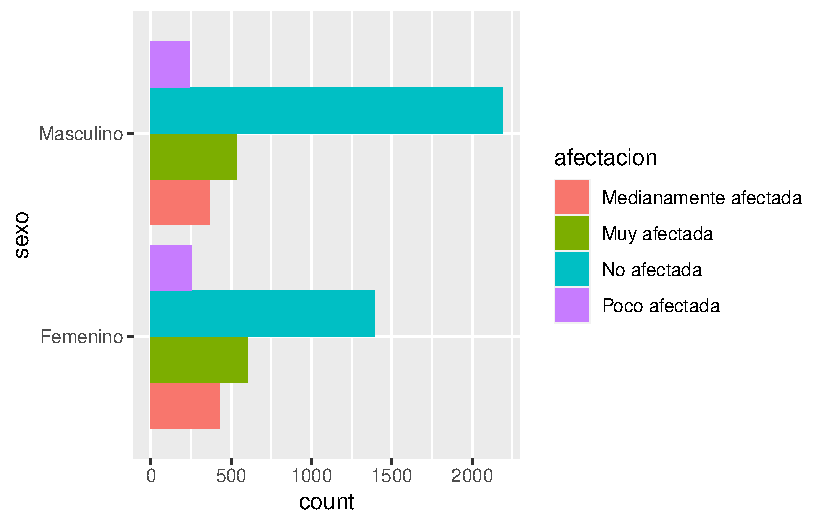
\includegraphics{notebook_visualization_files/figure-pdf/unnamed-chunk-5-1.pdf}

}

\end{figure}

\begin{center}\rule{0.5\linewidth}{0.5pt}\end{center}

\hypertarget{actividad}{%
\section{Actividad}\label{actividad}}

Repliquemos los gráficos en el siguiente enlace.

\href{https://ggplot2.tidyverse.org/reference/geom_bar.html}{Enlace acá}

\begin{center}\rule{0.5\linewidth}{0.5pt}\end{center}

\hypertarget{reflexiones-sobre-cuxf3mo-visualizar}{%
\section{Reflexiones sobre cómo
visualizar}\label{reflexiones-sobre-cuxf3mo-visualizar}}

La visualización, es en parte un arte y en parte una ciencia (Wilke,
2019).

La relevancia de la visualización se genera como una aproximación visual
resumida a los datos. El problema, es que no todas las visualizaciones
son buenas, en otras palabras no todos los gráficos son construidos de
manera correcta.

Un buen gráfico no responde necesariamente sobre el ¿cómo se ve?, sino
que debe responder a la necesidad de ¿quién lo ve? y ¿por qué lo ve?

\hypertarget{lo-que-no-se-debe-hacer-y-lo-que-se-debe-hacer.}{%
\subsection{Lo que no se debe hacer y lo que se debe
hacer.}\label{lo-que-no-se-debe-hacer-y-lo-que-se-debe-hacer.}}

Veamos un primer ejemplo:

\begin{figure}[H]

{\centering \includegraphics[width=0.5\textwidth,height=\textheight]{imagenes/graph_01.jpg}

}

\caption{Wilke (2019)}

\end{figure}

¿Qué le parece a usted? ¿es un buen o mal gráfico?

Otro ejemplo:

\begin{figure}[H]

{\centering \includegraphics[width=0.5\textwidth,height=\textheight]{imagenes/graph_02.jpg}

}

\caption{Wilke (2019)}

\end{figure}

\hypertarget{feo-malo-y-maluxedsimo-wilke-2019.}{%
\subsection{Feo, malo y malísimo (Wilke,
2019).}\label{feo-malo-y-maluxedsimo-wilke-2019.}}

Un gráfico puede tener tres errores:

\begin{itemize}
\item
  Feo (Ugly): falla la estética, pudiendo ser claro e informativo.
\item
  Malo (Bad): problemas de percepción en el gráfico, pudiendo ser poco
  claro, confuso o engañoso.
\item
  Malísimo (Wrong): existen errores matemáticos detrás del gráfico.
\end{itemize}

De manera aplicada:

\begin{figure}[H]

{\centering \includegraphics[width=0.7\textwidth,height=\textheight]{imagenes/graph_05.jpg}

}

\caption{Wilke (2019)}

\end{figure}

Un ejemplo más realista de lo antes mencionado. Este gráfico, ¿está feo,
malo o malísimo?

\begin{figure}[H]

{\centering \includegraphics[width=0.7\textwidth,height=\textheight]{imagenes/graph_06.jpg}

}

\caption{Evergreen (2019)}

\end{figure}

\hypertarget{la-intencionalidad-detruxe1s-del-gruxe1fico.}{%
\subsection{La intencionalidad detrás del
gráfico.}\label{la-intencionalidad-detruxe1s-del-gruxe1fico.}}

Dos maneras distintas de graficar lo mismo: una mejor que otra.

\begin{figure}[H]

{\centering \includegraphics[width=0.7\textwidth,height=\textheight]{imagenes/graph_03.jpg}

}

\caption{Evergreen (2019)}

\end{figure}

\begin{figure}[H]

{\centering \includegraphics[width=0.5\textwidth,height=\textheight]{imagenes/graph_04.jpg}

}

\caption{Evergreen (2019)}

\end{figure}

\hypertarget{la-visualizaciuxf3n-ideal-en-seis-imaguxe9nes-roam-2016.}{%
\section{La visualización ideal en seis imagénes (Roam,
2016).}\label{la-visualizaciuxf3n-ideal-en-seis-imaguxe9nes-roam-2016.}}

\begin{enumerate}
\def\labelenumi{\arabic{enumi}.}
\item
  Who and what is involved (¿Quién o qué está involucrado?): Se debe
  iniciar con un resumen visual sobre lo que se hablará.
\item
  How many are involved (¿Qué cantidad está involucrada?): Se deben
  generar medidas cuantitativas de lo hablado. Cambios en los números
  también son relevantes.
\item
  Where the pieces are located (¿Dónde se ubica?): Presentar alguna
  relación visual entre lo hablado y su ubicación.
\item
  When things occur (¿Cuándo ocurre?): Mostrar algo relacionado con la
  temporalidad o la secuencia de los eventos en las que ocurren las
  interacciones relevantes.
\item
  How things impact each other (¿Cómo las cosas se relacionan?): Generar
  una visualización que presente la relación causa - efecto que afectan
  lo mostrado anteriormente.
\item
  Why this matters (¿Por qué es importante?): Se debe concluir
  visualizado anteriormente.
\end{enumerate}

\begin{figure}[H]

{\centering \includegraphics[width=0.7\textwidth,height=\textheight]{imagenes/imagen_61.jpg}

}

\caption{Evergreen (2019)}

\end{figure}

\hypertarget{storytelling-with-data}{%
\section{Storytelling with data}\label{storytelling-with-data}}

Seis puntos claves:

\begin{enumerate}
\def\labelenumi{\arabic{enumi}.}
\tightlist
\item
  Comprender el contexto
\item
  Elegir el gráfico adecuado
\item
  Eliminar el caos
\item
  Dirija la atención hacía donde le interese
\item
  Piense como un diseñador
\item
  Cuente una historia
\end{enumerate}

En relación a este enfoque, se puede consutar el siguiente material:

\href{https://www.storytellingwithdata.com}{Página del libro}

\hypertarget{referencias}{%
\section{Referencias}\label{referencias}}

\begin{itemize}
\item
  Wilke, C. O. (2019). Fundamentals of data visualization: a primer on
  making informative and compelling figures. O'Reilly Media.
\item
  Evergreen, S. D. (2019). Effective data visualization: The right chart
  for the right data. SAGE publications.
\end{itemize}



\end{document}
